% Options for packages loaded elsewhere
\PassOptionsToPackage{unicode}{hyperref}
\PassOptionsToPackage{hyphens}{url}
%
\documentclass[
]{article}
\usepackage{amsmath,amssymb}
\usepackage{lmodern}
\usepackage{iftex}
\ifPDFTeX
  \usepackage[T1]{fontenc}
  \usepackage[utf8]{inputenc}
  \usepackage{textcomp} % provide euro and other symbols
\else % if luatex or xetex
  \usepackage{unicode-math}
  \defaultfontfeatures{Scale=MatchLowercase}
  \defaultfontfeatures[\rmfamily]{Ligatures=TeX,Scale=1}
\fi
% Use upquote if available, for straight quotes in verbatim environments
\IfFileExists{upquote.sty}{\usepackage{upquote}}{}
\IfFileExists{microtype.sty}{% use microtype if available
  \usepackage[]{microtype}
  \UseMicrotypeSet[protrusion]{basicmath} % disable protrusion for tt fonts
}{}
\makeatletter
\@ifundefined{KOMAClassName}{% if non-KOMA class
  \IfFileExists{parskip.sty}{%
    \usepackage{parskip}
  }{% else
    \setlength{\parindent}{0pt}
    \setlength{\parskip}{6pt plus 2pt minus 1pt}}
}{% if KOMA class
  \KOMAoptions{parskip=half}}
\makeatother
\usepackage{xcolor}
\IfFileExists{xurl.sty}{\usepackage{xurl}}{} % add URL line breaks if available
\IfFileExists{bookmark.sty}{\usepackage{bookmark}}{\usepackage{hyperref}}
\hypersetup{
  pdftitle={About},
  hidelinks,
  pdfcreator={LaTeX via pandoc}}
\urlstyle{same} % disable monospaced font for URLs
\usepackage[margin=1in]{geometry}
\usepackage{longtable,booktabs,array}
\usepackage{calc} % for calculating minipage widths
% Correct order of tables after \paragraph or \subparagraph
\usepackage{etoolbox}
\makeatletter
\patchcmd\longtable{\par}{\if@noskipsec\mbox{}\fi\par}{}{}
\makeatother
% Allow footnotes in longtable head/foot
\IfFileExists{footnotehyper.sty}{\usepackage{footnotehyper}}{\usepackage{footnote}}
\makesavenoteenv{longtable}
\usepackage{graphicx}
\makeatletter
\def\maxwidth{\ifdim\Gin@nat@width>\linewidth\linewidth\else\Gin@nat@width\fi}
\def\maxheight{\ifdim\Gin@nat@height>\textheight\textheight\else\Gin@nat@height\fi}
\makeatother
% Scale images if necessary, so that they will not overflow the page
% margins by default, and it is still possible to overwrite the defaults
% using explicit options in \includegraphics[width, height, ...]{}
\setkeys{Gin}{width=\maxwidth,height=\maxheight,keepaspectratio}
% Set default figure placement to htbp
\makeatletter
\def\fps@figure{htbp}
\makeatother
\setlength{\emergencystretch}{3em} % prevent overfull lines
\providecommand{\tightlist}{%
  \setlength{\itemsep}{0pt}\setlength{\parskip}{0pt}}
\setcounter{secnumdepth}{5}
\usepackage{booktabs}
\ifLuaTeX
  \usepackage{selnolig}  % disable illegal ligatures
\fi
\usepackage[]{natbib}
\bibliographystyle{plainnat}

\title{About}
\usepackage{etoolbox}
\makeatletter
\providecommand{\subtitle}[1]{% add subtitle to \maketitle
  \apptocmd{\@title}{\par {\large #1 \par}}{}{}
}
\makeatother
\subtitle{An company focused on applying open source tools for small business support.}
\author{}
\date{\vspace{-2.5em}2022-03-20}

\usepackage{amsthm}
\newtheorem{theorem}{Theorem}[section]
\newtheorem{lemma}{Lemma}[section]
\newtheorem{corollary}{Corollary}[section]
\newtheorem{proposition}{Proposition}[section]
\newtheorem{conjecture}{Conjecture}[section]
\theoremstyle{definition}
\newtheorem{definition}{Definition}[section]
\theoremstyle{definition}
\newtheorem{example}{Example}[section]
\theoremstyle{definition}
\newtheorem{exercise}{Exercise}[section]
\theoremstyle{definition}
\newtheorem{hypothesis}{Hypothesis}[section]
\theoremstyle{remark}
\newtheorem*{remark}{Remark}
\newtheorem*{solution}{Solution}
\begin{document}
\maketitle

{
\setcounter{tocdepth}{2}
\tableofcontents
}
\hypertarget{hello-bookdown}{%
\section{Hello bookdown}\label{hello-bookdown}}

All chapters start with a first-level heading followed by your chapter title, like the line above. There should be only one first-level heading (\texttt{\#}) per .Rmd file.

\hypertarget{a-section}{%
\subsection{A section}\label{a-section}}

All chapter sections start with a second-level (\texttt{\#\#}) or higher heading followed by your section title, like the sections above and below here. You can have as many as you want within a chapter.

\hypertarget{an-unnumbered-section}{%
\subsubsection*{An unnumbered section}\label{an-unnumbered-section}}
\addcontentsline{toc}{subsubsection}{An unnumbered section}

Chapters and sections are numbered by default. To un-number a heading, add a \texttt{\{.unnumbered\}} or the shorter \texttt{\{-\}} at the end of the heading, like in this section.

--\textgreater{}
--\textgreater{}

--\textgreater{}

--\textgreater{}

--\textgreater{}

--\textgreater{}
--\textgreater{}

\href{https://discordapp.com/widget?id=944005450830077992\&theme=dark}{
\includegraphics{statisticsnetwork_files/figure-latex/unnamed-chunk-3-1.pdf}}

Any enquires welcome!

{[}1{]} S. Benjamins, W. Ledwell, J. Huntington, et al.~``Assessing changes
in numbers and distribution of large whale entanglements in
Newfoundland and Labrador, Canada1''. In: \emph{Marine Mammal Science} 28.3
(Jul.~2012), pp.~579-601. ISSN: 08240469. DOI:
10.1111/j.1748-7692.2011.00511.x. \textless URL:
\url{https://onlinelibrary.wiley.com/doi/10.1111/j.1748-7692.2011.00511.x}\textgreater{}
(visited on 03/17/2022).

{[}2{]} A. R. Davidson, W. Rayment, S. M. Dawson, et al.~``Estimated calving
interval for the New Zealand southern right whale (Eubalaena
australis)''. In: \emph{New Zealand Journal of Marine and Freshwater
Research} 52.3 (2018), pp.~372-382. ISSN: 0028-8330. DOI:
10.1080/00288330.2017.1397034. \textless URL:
\url{https://doi.org/10.1080/00288330.2017.1397034}\textgreater{} (visited on 11/27/2018).

{[}3{]} M. Medina‐Romero, A. O'Reilly‐Nugent, A. Davidson, et al.~``Effect
of detection heterogeneity in occupancy‐detection models: an
experimental test of time‐to‐first‐detection methods''. In:
\emph{Ecography} (May. 20, 2019). Citation Key Alias:
medina-romeroEffectDetectionHeterogeneity2019,
medina-romeroEffectDetectionHeterogeneity2019b,
medina-romeroEffectDetectionHeterogeneity2019c,
medina-romeroEffectDetectionHeterogeneity2019d,
medina-romeroEffectDetectionHeterogeneity2019e, p.~ecog.04321. ISSN:
0906-7590, 1600-0587. DOI: 10.1111/ecog.04321. \textless URL:
\url{https://onlinelibrary.wiley.com/doi/abs/10.1111/ecog.04321}\textgreater{} (visited on
06/03/2019).

{[}4{]} S. Meyer, A. R. Davidson, M. Krkošek, et al.~``Comment on
‘Current bycatch levels in Auckland Islands trawl fisheries unlikely
to be driving New Zealand sea lion \textit(Phocarctos hookeri)
population decline’: COMMENT ON HAMILTON \& BAKER (2014)''. In:
\emph{Aquatic Conserv: Mar.~Freshw. Ecosyst.} 25.4 (Aug.~2015), pp.~584-586.
ISSN: 10527613. DOI: 10.1002/aqc.2567. \textless URL:
\url{https://onlinelibrary.wiley.com/doi/10.1002/aqc.2567}\textgreater{} (visited on
03/17/2022).

{[}5{]} W. Rayment, A. Davidson, S. Dawson, et al.~``Distribution of
southern right whales on the Auckland Islands calving grounds''. In:
\emph{New Zealand Journal of Marine and Freshwater Research} 46.3 (Sep.
2012), pp.~431-436. ISSN: 0028-8330, 1175-8805. DOI:
10.1080/00288330.2012.697072. \textless URL:
\url{http://www.tandfonline.com/doi/abs/10.1080/00288330.2012.697072}\textgreater{}
(visited on 03/17/2022).

\hypertarget{hello-bookdown-1}{%
\section{Hello bookdown}\label{hello-bookdown-1}}

All chapters start with a first-level heading followed by your chapter title, like the line above. There should be only one first-level heading (\texttt{\#}) per .Rmd file.

\hypertarget{a-section-1}{%
\subsection{A section}\label{a-section-1}}

All chapter sections start with a second-level (\texttt{\#\#}) or higher heading followed by your section title, like the sections above and below here. You can have as many as you want within a chapter.

\hypertarget{an-unnumbered-section-1}{%
\subsubsection*{An unnumbered section}\label{an-unnumbered-section-1}}
\addcontentsline{toc}{subsubsection}{An unnumbered section}

Chapters and sections are numbered by default. To un-number a heading, add a \texttt{\{.unnumbered\}} or the shorter \texttt{\{-\}} at the end of the heading, like in this section.

\hypertarget{cross}{%
\section{Cross-references}\label{cross}}

Cross-references make it easier for your readers to find and link to elements in your book.

\hypertarget{chapters-and-sub-chapters}{%
\subsection{Chapters and sub-chapters}\label{chapters-and-sub-chapters}}

There are two steps to cross-reference any heading:

\begin{enumerate}
\def\labelenumi{\arabic{enumi}.}
\tightlist
\item
  Label the heading: \texttt{\#\ Hello\ world\ \{\#nice-label\}}.

  \begin{itemize}
  \tightlist
  \item
    Leave the label off if you like the automated heading generated based on your heading title: for example, \texttt{\#\ Hello\ world} = \texttt{\#\ Hello\ world\ \{\#hello-world\}}.
  \item
    To label an un-numbered heading, use: \texttt{\#\ Hello\ world\ \{-\#nice-label\}} or \texttt{\{\#\ Hello\ world\ .unnumbered\}}.
  \end{itemize}
\item
  Next, reference the labeled heading anywhere in the text using \texttt{\textbackslash{}@ref(nice-label)}; for example, please see Chapter \ref{cross}.

  \begin{itemize}
  \tightlist
  \item
    If you prefer text as the link instead of a numbered reference use: \protect\hyperlink{cross}{any text you want can go here}.
  \end{itemize}
\end{enumerate}

\hypertarget{captioned-figures-and-tables}{%
\subsection{Captioned figures and tables}\label{captioned-figures-and-tables}}

Figures and tables \emph{with captions} can also be cross-referenced from elsewhere in your book using \texttt{\textbackslash{}@ref(fig:chunk-label)} and \texttt{\textbackslash{}@ref(tab:chunk-label)}, respectively.

See Figure \ref{fig:nice-fig}.

\begin{figure}

{\centering 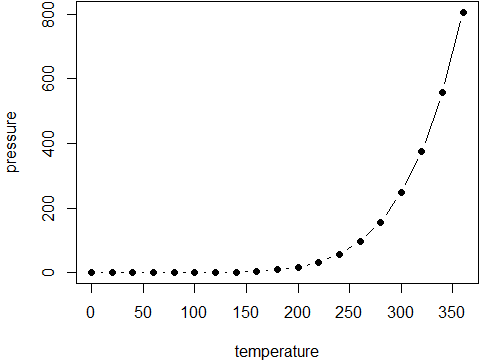
\includegraphics[width=0.8\linewidth]{statisticsnetwork_files/figure-latex/nice-fig-1} 

}

\caption{Here is a nice figure!}\label{fig:nice-fig}
\end{figure}

Don't miss Table \ref{tab:nice-tab}.

\begin{table}

\caption{\label{tab:nice-tab}Here is a nice table!}
\centering
\begin{tabular}[t]{rr}
\toprule
temperature & pressure\\
\midrule
0 & 0.0002\\
20 & 0.0012\\
40 & 0.0060\\
60 & 0.0300\\
80 & 0.0900\\
\addlinespace
100 & 0.2700\\
120 & 0.7500\\
140 & 1.8500\\
160 & 4.2000\\
180 & 8.8000\\
\bottomrule
\end{tabular}
\end{table}

\hypertarget{parts}{%
\section{Parts}\label{parts}}

You can add parts to organize one or more book chapters together. Parts can be inserted at the top of an .Rmd file, before the first-level chapter heading in that same file.

Add a numbered part: \texttt{\#\ (PART)\ Act\ one\ \{-\}} (followed by \texttt{\#\ A\ chapter})

Add an unnumbered part: \texttt{\#\ (PART\textbackslash{}*)\ Act\ one\ \{-\}} (followed by \texttt{\#\ A\ chapter})

Add an appendix as a special kind of un-numbered part: \texttt{\#\ (APPENDIX)\ Other\ stuff\ \{-\}} (followed by \texttt{\#\ A\ chapter}). Chapters in an appendix are prepended with letters instead of numbers.

\hypertarget{footnotes-and-citations}{%
\section{Footnotes and citations}\label{footnotes-and-citations}}

\hypertarget{footnotes}{%
\subsection{Footnotes}\label{footnotes}}

Footnotes are put inside the square brackets after a caret \texttt{\^{}{[}{]}}. Like this one \footnote{This is a footnote.}.

\hypertarget{citations}{%
\subsection{Citations}\label{citations}}

Reference items in your bibliography file(s) using \texttt{@key}.

For example, we are using the \textbf{bookdown} package \citep{R-bookdown} (check out the last code chunk in index.Rmd to see how this citation key was added) in this sample book, which was built on top of R Markdown and \textbf{knitr} \citep{xie2015} (this citation was added manually in an external file book.bib).
Note that the \texttt{.bib} files need to be listed in the index.Rmd with the YAML \texttt{bibliography} key.

The RStudio Visual Markdown Editor can also make it easier to insert citations: \url{https://rstudio.github.io/visual-markdown-editing/\#/citations}

\hypertarget{blocks}{%
\section{Blocks}\label{blocks}}

\hypertarget{equations}{%
\subsection{Equations}\label{equations}}

Here is an equation.

\begin{equation} 
  f\left(k\right) = \binom{n}{k} p^k\left(1-p\right)^{n-k}
  \label{eq:binom}
\end{equation}

You may refer to using \texttt{\textbackslash{}@ref(eq:binom)}, like see Equation \eqref{eq:binom}.

\hypertarget{theorems-and-proofs}{%
\subsection{Theorems and proofs}\label{theorems-and-proofs}}

Labeled theorems can be referenced in text using \texttt{\textbackslash{}@ref(thm:tri)}, for example, check out this smart theorem \ref{thm:tri}.

\begin{theorem}
\protect\hypertarget{thm:tri}{}\label{thm:tri}For a right triangle, if \(c\) denotes the \emph{length} of the hypotenuse
and \(a\) and \(b\) denote the lengths of the \textbf{other} two sides, we have
\[a^2 + b^2 = c^2\]
\end{theorem}

Read more here \url{https://bookdown.org/yihui/bookdown/markdown-extensions-by-bookdown.html}.

\hypertarget{callout-blocks}{%
\subsection{Callout blocks}\label{callout-blocks}}

The R Markdown Cookbook provides more help on how to use custom blocks to design your own callouts: \url{https://bookdown.org/yihui/rmarkdown-cookbook/custom-blocks.html}

Appying for jobs in a post-Covid world could be very different but one key aspect is to be able to communicate the skills needed to be employable. Here is a invovative way of including interactive rmarkdown files into my graduate CV to demostrate the skills I have throughout the scientific process through my training and previous experinence.

\hypertarget{rmarkdown}{%
\subsection{Rmarkdown}\label{rmarkdown}}

Over the duration of my PhD I have developed a collection of scientific computing skills that lie within the scope of computational reproducibility. Coincidently, these tools are the same basic functionality to website development.

For more information about simple R Markdown websites, please read the documentation at \url{https://bookdown.org/yihui/rmarkdown/rmarkdown-site.html}.

Please also note that simple R Markdown sites are \emph{not} based on \textbf{blogdown}. They are probably good for websites with only a few Rmd documents. For larger-scale and more sophisticated websites (such as blogs), you may want to use \textbf{blogdown} instead: \url{https://github.com/rstudio/blogdown}.

This is the base Jekyll theme combined with the html5 template here and build in rmarkdown through RStudio.

\hypertarget{jekyll}{%
\subsection{Jekyll}\label{jekyll}}

You can find out more info about customizing your Jekyll theme, as well as basic Jekyll usage documentation at jekyllrb.com

You can find the source code for Minima at GitHub:
jekyll /
minima

You can find the source code for Jekyll at \href{https://github.com/jekyll/jekyll}{GitHub}

{[}jekyll-organization{]}: \url{https://github.com/jekyll}

\hypertarget{contact}{%
\subsection{Contact}\label{contact}}

\hypertarget{publishing}{%
\subsection{Publishing}\label{publishing}}

HTML books can be published online, see: \url{https://bookdown.org/yihui/bookdown/publishing.html}

\hypertarget{pages}{%
\subsection{404 pages}\label{pages}}

By default, users will be directed to a 404 page if they try to access a webpage that cannot be found. If you'd like to customize your 404 page instead of using the default, you may add either a \texttt{\_404.Rmd} or \texttt{\_404.md} file to your project root and use code and/or Markdown syntax.

\hypertarget{metadata-for-sharing}{%
\subsection{Metadata for sharing}\label{metadata-for-sharing}}

Bookdown HTML books will provide HTML metadata for social sharing on platforms like Twitter, Facebook, and LinkedIn, using information you provide in the \texttt{index.Rmd} YAML. To setup, set the \texttt{url} for your book and the path to your \texttt{cover-image} file. Your book's \texttt{title} and \texttt{description} are also used.

This \texttt{gitbook} uses the same social sharing data across all chapters in your book- all links shared will look the same.

Specify your book's source repository on GitHub using the \texttt{edit} key under the configuration options in the \texttt{\_output.yml} file, which allows users to suggest an edit by linking to a chapter's source file.

Read more about the features of this output format here:

\url{https://pkgs.rstudio.com/bookdown/reference/gitbook.html}

Or use:

We are really glad you're reading this! We need volunteer contributors for making the statistics network successful. Please do not hesitate to contact us via any way works best for you.

\hypertarget{contributing-with-version-control}{%
\subsection{Contributing with version control}\label{contributing-with-version-control}}

\{: style=``text-align: justify''\}

Making contribution is simple with git following these steps:

\begin{enumerate}
\def\labelenumi{\arabic{enumi}.}
\tightlist
\item
  Fork the repo on GitHub \href{https://github.com/davan690/davan690.github.io}{here}
\item
  Clone the project to your own machine
\item
  Edit the files or add files using your favorite editor
\item
  Commit changes to your own branch
\item
  Push your work back up to your fork
\item
  Submit a Pull request so that we can review your changes
\end{enumerate}

NOTE: Be sure to merge the latest from ``upstream'' before making a pull request!
\{: style=``text-align: justify''\}

If you're comfortable making contributions any other way, please feel free to do it your way and send us the pull request, message or email and we will gladly review the changes.

\href{mailto:anthony.davidson@canberra.edu.au}{\nolinkurl{anthony.davidson@canberra.edu.au}}
statisticsnetwork
statisticsnetwork

  \bibliography{book.bib,packages.bib}

\end{document}
